Example 1: 
Create LShape reinforcement in structural element.
\begin{figure}[H] 
	\centering 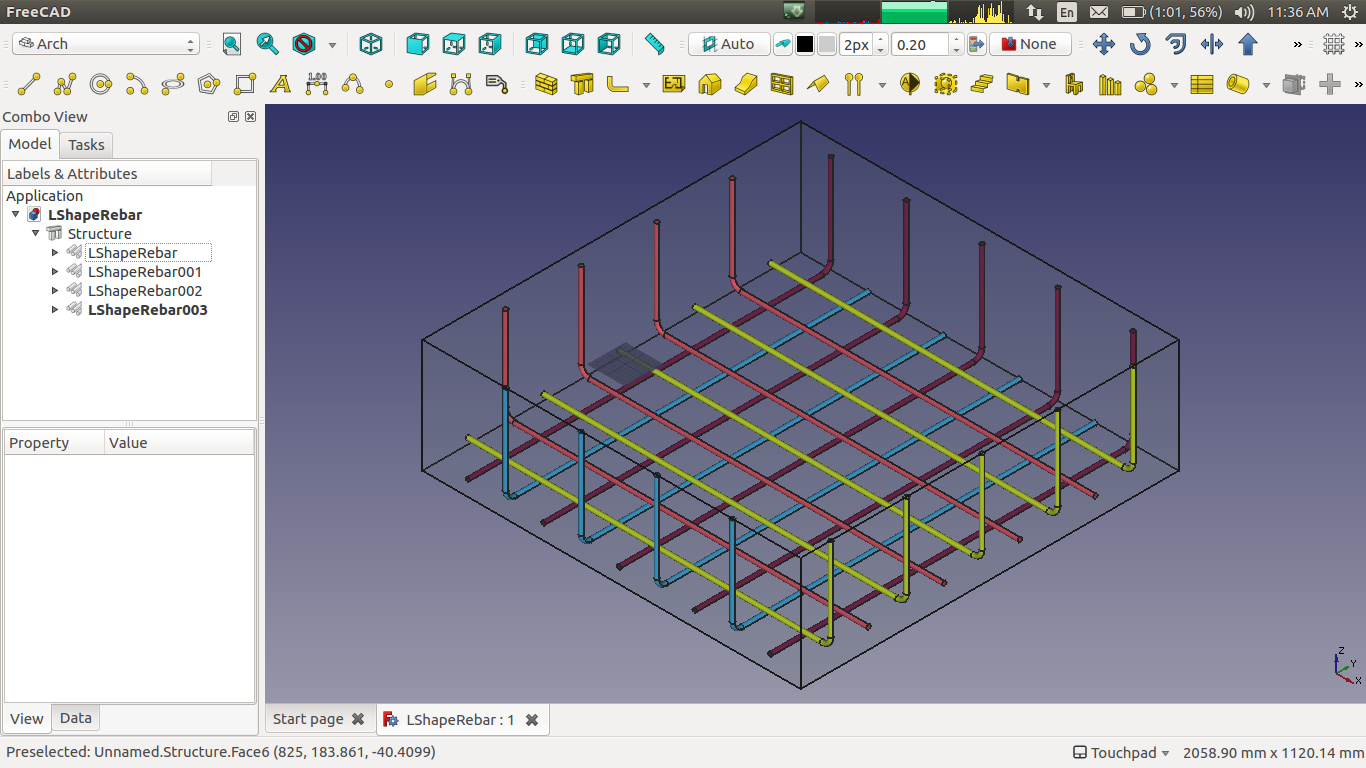
\includegraphics[scale=0.31]{images/LShapeRebarNew.png}
	\caption{LShape reinforcing bar in the structural element.}
\end{figure}

%\begin{lstlisting}[language=python]
\begin{verbatim}
# Creating LShape rebar.
import Arch, LShapeRebar
structure = Arch.makeStructure(length=1000.0, width=1000.0, height=400.0)
structure.ViewObject.Transparency = 80
FreeCAD.ActiveDocument.recompute()
rebar = LShapeRebar.makeLShapeRebar(20, 20, 20, 20, 8, 20, 2, True,\
    10, "Bottom Left", structure, "Face1") 

# Changing properties of LShape rebar.
import LShapeRebar
LShapeRebar.editLShapeRebar(50, 50, 20, 20, 8, 20, 2, True, 5, "Top Left")

# Written by Amritpal Singh <amrit3701@gmail.com>
#
# To the extent possible under law, the author(s) have dedicated all
# copyright and related and neighboring rights to this software to the
# public domain worldwide. This software is distributed without any
# warranty.
#
# You should have received a copy of the CC0 Public Domain
# Dedication along with this software.
# If not, see <http://creativecommons.org/publicdomain/zero/1.0/>.
\end{verbatim}

